% Paquets généraux
\documentclass[a4paper,12pt,titlepage]{article}
\usepackage[T1]{fontenc}
\usepackage[utf8]{inputenc}
\usepackage[french]{babel}
\usepackage[gen]{eurosym}
%\usepackage[dvips]{graphicx}
\usepackage{fancyhdr}
\usepackage{pdfpages} 
\usepackage{multido}
\usepackage{hyperref}
%\usepackage{textcomp}
%\usepackage{aeguill}
\usepackage{schemabloc}
\usepackage[bitstream-charter]{mathdesign}
\usepackage{pstricks}
\usepackage{helvet}

\newcommand{\id}{71}
\newcommand{\nom}{Théorie des mécanismes}
\newcommand{\sequence}{04}
\newcommand{\nomsequence}{Liaisons entre les solides}
\newcommand{\num}{02}
\newcommand{\type}{KH}
\newcommand{\descrip}{Liaisons équivalentes, hyperstatisme, liaisons en série et en parallèle, théorie des graphes}
\newcommand{\competences}{B2-12: Proposer une modélisation des liaisons avec leurs caractéristiques géométriques. \\ &  B2-13: Proposer un modèle cinématique paramétré à partir d'un système réel, d'une maquette numérique ou d'u \\ &  B2-17: Simplifier un modèle de mécanisme. \\ &  B2-18: Modifier un modèle pour le rendre isostatique. \\ &  C1-04: Proposer une démarche permettant d'obtenir une loi entrée-sortie géométrique.  \\ &  C2-05: Caractériser le mouvement d'un repère par rapport à un autre repère. \\ &  C2-06: Déterminer les relations entre les grandeurs géométriques ou cinématiques. }
\newcommand{\nbcomp}{7}
\newcommand{\systemes}{}
\newcommand{\systemesnum}{}
\newcommand{\systemessansaccent}{}
\newcommand{\ilot}{2}
\newcommand{\ilotstr}{02}
\newcommand{\dossierilot}{\detokenize{Ilot_02 }}


\newcommand{\auteurun}{Renaud Costadoat}
\newcommand{\institute}{Lycée Dorian}


\usepackage{color}
\usepackage{xcolor}
\usepackage{colortbl}
\usepackage{helvet}
\renewcommand{\familydefault}{\sfdefault}
\usepackage{amsfonts}
\usepackage{amsmath}
%\usepackage{xspace}
\usepackage{varioref}
\usepackage{tabularx}
%\usepackage{floatflt}
\usepackage{graphics}
\usepackage{wrapfig}
\usepackage{textcomp}
\usepackage{tikz}
\usepackage{wrapfig}
\usepackage{gensymb}
\usepackage[european]{circuitikz}
\usetikzlibrary{babel}
\usepackage{ifthen}
\usepackage{cancel}
\usepackage{etoolbox}
\usepackage{multirow}
%\usepackage{boxedminipage}
\definecolor{gris25}{gray}{0.75}
\definecolor{bleu}{RGB}{18,33,98}
\definecolor{bleuf}{RGB}{42,94,171}
\definecolor{bleuc}{RGB}{231,239,247}
\definecolor{rougef}{RGB}{185,18,27}
\definecolor{rougec}{RGB}{255,188,204}%255,230,231
\definecolor{vertf}{RGB}{103,126,82}
\definecolor{vertc}{RGB}{220,255,191}
\definecolor{forestgreen}{rgb}{0.13,0.54,0.13}
\definecolor{blcr}{rgb}{0.59,0.69,0.84}
\definecolor{blfr}{rgb}{0.32,0.51,0.75}
\definecolor{orfr}{rgb}{0.90,0.42,0.15}
\definecolor{orcr}{rgb}{0.90,0.65,0.50}
\definecolor{orangef}{rgb}{0.659,0.269,0.072}
\definecolor{orange}{rgb}{0.58,0.35,0.063}
\definecolor{orangec}{rgb}{0.43,0.32,0.25}
\definecolor{rcorrect}{rgb}{0.6,0,0}
\definecolor{sequence}{rgb}{0.75,0.75,0.75}
\definecolor{competences}{rgb}{0.61,0.73,0.35}
\definecolor{grisf}{HTML}{222222}
\definecolor{grisc}{HTML}{636363}
\definecolor{normal}{HTML}{4087c4}
\definecolor{info}{HTML}{5bc0de}
\definecolor{success}{RGB}{92,184,92}
\definecolor{warning}{RGB}{240,173,78}
\definecolor{danger}{RGB}{217,83,79}
\hypersetup{                    % parametrage des hyperliens
    colorlinks=true,                % colorise les liens
    breaklinks=true,                % permet les retours à la ligne pour les liens trop longs
    urlcolor= blfr,                 % couleur des hyperliens
    linkcolor= orange,                % couleur des liens internes aux documents (index, figures, tableaux, equations,...)
    citecolor= forestgreen                % couleur des liens vers les references bibliographiques
    }

% Mise en page
\pagestyle{fancy}

\setlength{\hoffset}{-18pt}

\setlength{\oddsidemargin}{0pt} 	% Marge gauche sur pages impaire2s
\setlength{\evensidemargin}{0pt} 	% Marge gauche sur pages paires
\setlength{\marginparwidth}{00pt} 	% Largeur de note dans la marge
\setlength{\headwidth}{481pt} 	 	% Largeur de la zone de tête (17cm)
\setlength{\textwidth}{481pt} 	 	% Largeu\textbf{r de la zone de texte (17cm)
\setlength{\voffset}{-18pt} 		% Bon pour DOS
\setlength{\marginparsep}{7pt}	 	% Séparation de la marge
\setlength{\topmargin}{-30pt} 		% Pas de marge en haut
\setlength{\headheight}{55pt} 		% Haut de page
\setlength{\headsep}{20pt} 		% Entre le haut de page et le texte
\setlength{\footskip}{30pt} 		% Bas de\textbf{ page + séparation
\setlength{\textheight}{700pt} 		% Hauteur de l'icone zone de texte (25cm)
\setlength\fboxrule{1 pt}
\renewcommand{\baselinestretch}{1}
\setcounter{tocdepth}{1}
\newcommand{\cadre}[2]
{\fbox{
  \begin{minipage}{#1\linewidth}
   \begin{center}
    #2\\
   \end{center}
  \end{minipage}
 }
}


\newcommand{\titre}[1]
{\begin{center}
\cadre{0.8}{\huge #1} 
\end{center}
}

\newcounter{num_quest} \setcounter{num_quest}{0}
\newcounter{num_rep} \setcounter{num_rep}{0}

\newcommand{\question}[1]{\refstepcounter{num_quest}\par
~\ \\ \textbf{Question \arabic{num_quest} : }#1\label{q\the\value{num_quest}}\par
}

\newcommand{\reponse}[1]
{\noindent
\rule{\linewidth}{.5pt}\\
\textbf{Question \refstepcounter{num_rep}\ref{q\the\value{num_rep}} :} ~\ \\
#1}

% En tête et pied de page
\lhead{\nom}
\rhead{
\includegraphics[width=2cm]{../../img/logo}}
\lfoot{Renaud Costadoat}
\cfoot{Page \thepage}

\fancypagestyle{correction}{%
  \fancyhf{}
  \lhead{\colorbox{danger}{\begin{minipage}{0.65\paperwidth} \textcolor{white}{\textbf{Correction}} \end{minipage}} }
  \rhead{
\includegraphics[width=2cm]{../../img/logo}}
  \lfoot{Renaud Costadoat}
  \rfoot{\colorbox{danger}{\begin{minipage}{0.6\paperwidth} \begin{flushright}\textcolor{white}{\textbf{Correction}}\end{flushright} \end{minipage}} }}

\renewcommand{\footrulewidth}{0.4pt}

\usepackage{eso-pic}
\newcommand{\BackgroundPic}{%
\put(0,0){%
\parbox[b][\paperheight]{\paperwidth}{%
\vfill
\begin{center}
\hspace{0.5cm}\vspace{0.5cm}

\includegraphics[width=\paperwidth,height=\paperheight,%
keepaspectratio]{../../img/fond3}%
\end{center}
\vfill
}}}

\newcommand{\BackgroundPicdeux}{%
\put(25,-30){%
\parbox[b][\paperheight]{\paperwidth}{%
\vfill
\begin{center}
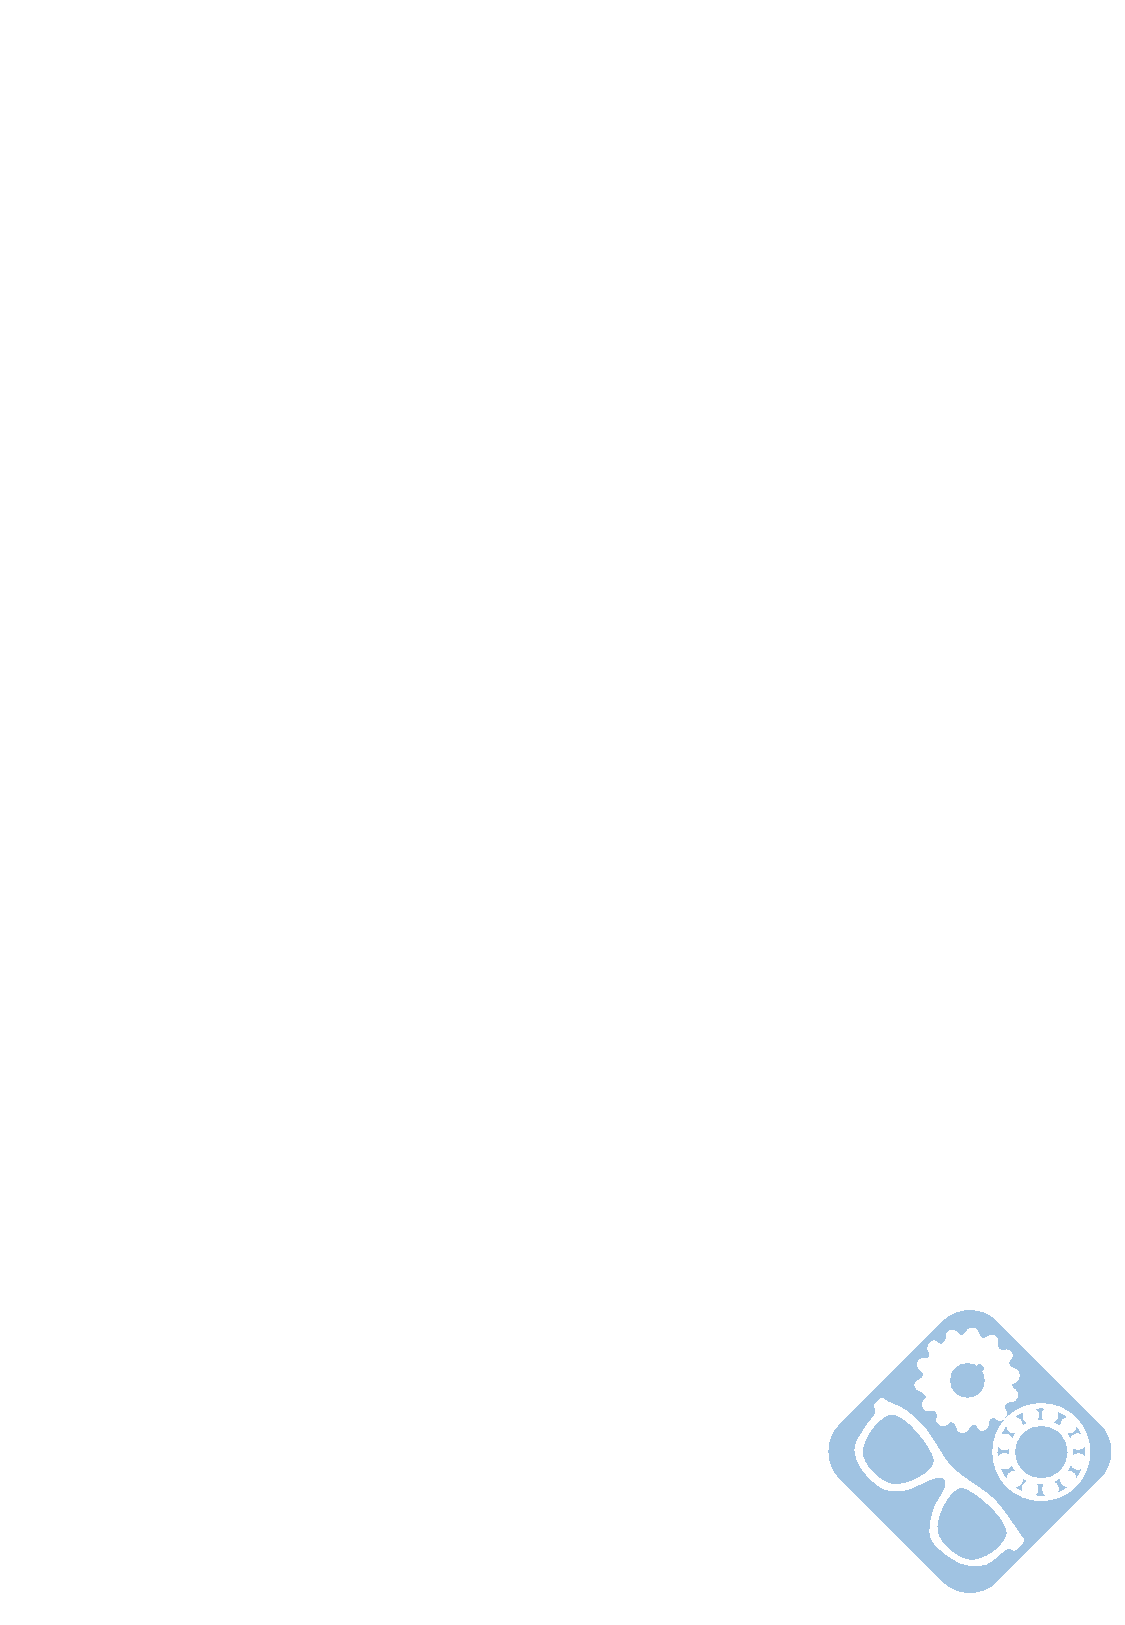
\includegraphics[width=\paperwidth,height=\paperheight,%
keepaspectratio]{../../img/fond4}%
\end{center}
\vfill
}}}

\begin{document}

\AddToShipoutPicture{\BackgroundPicdeux}

\pagestyle{fancy}

\section{Hacheur série pour porte de garage}

\subsection{Présentation}

\begin{minipage}{0.6\linewidth}
Le support de cet exercice est une porte automatique de garage collectif dans un immeuble. Le
synoptique concernant la partie électrique et une vue d'ensemble du dispositif sont donnés ci-dessous.
\end{minipage}\hfill
\begin{minipage}{0.35\linewidth}
\begin{center}
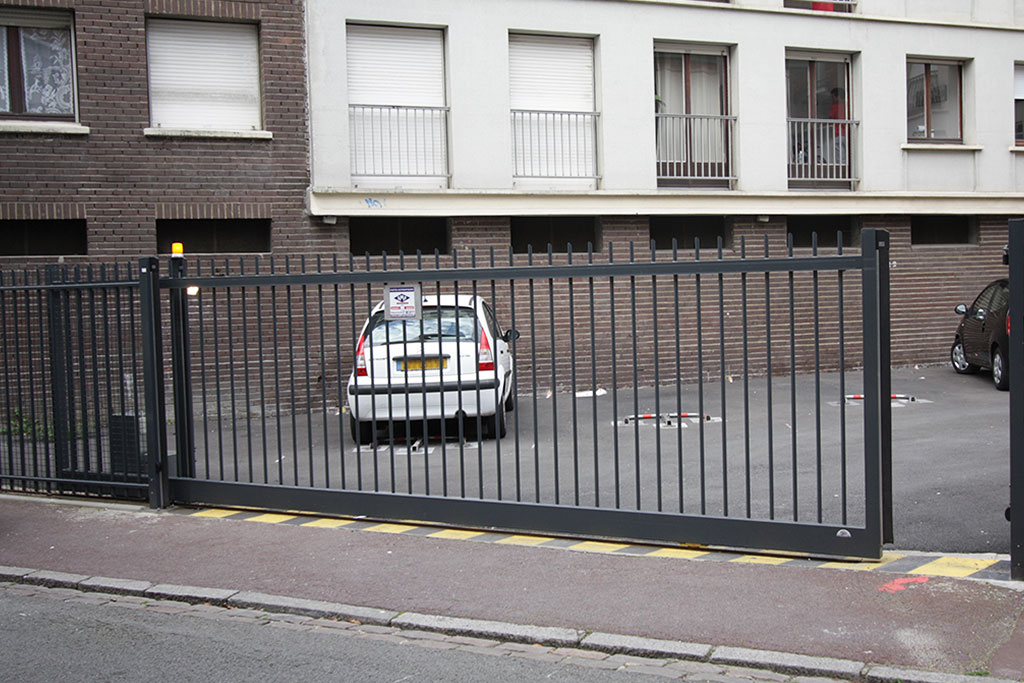
\includegraphics[width=.9\linewidth]{img/fig01}
\end{center}
\end{minipage}

~\

La tension d'alimentation du hacheur série est constante et vaut $V_S = 210 V$. $D$ est une diode idéale sans seuil. $K$ est un interrupteur parfait commandé
par une tension (voir figure \ref{schema_elec}).

\begin{figure}[ht!]
\begin{center}
 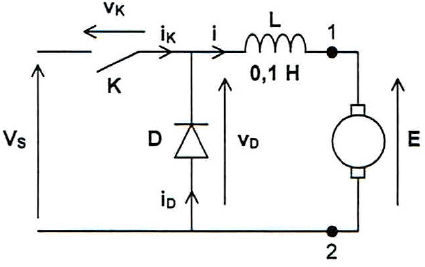
\includegraphics[width=.6\linewidth]{img/schema_elec}
\end{center}
\caption{\label{schema_elec}Schéma électrique du système}
\end{figure}

On note $\alpha$ le rapport cyclique de commande de ce hacheur et $T$ la période de fonctionnement:
\begin{itemize}
 \item Pour $t\in [0,\alpha\cdot T]$, $K$ est fermé,
 \item Pour $t\in [\alpha\cdot T, T]$, $K$ est ouvert.
\end{itemize}

On donne $T = 0,1 ms$.

E proportionnelle à la vitesse de rotation du moteur : $E = kN$ avec $k = 5,25\cdot 10^{-2} V\cdot tr^{-1}\cdot min$.

On suppose que l'intensité $i$ du courant ne s'annule jamais et varie entre les valeurs minimale et maximale $I_m$ et $I_M$.

D'après un exercice du Lycée Jean Zay (Thiers).

\subsection{Travail demandé}

\question{Déterminer l'expression de $i(t)$ en fonction de $V_S$, $E$, $L$ et $I_m$ pour $t\in [0, \alpha\cdot T]$ puis pour $t\in [\alpha\cdot T,T]$ en fonction de $E$, $L$ et $I_M$.}

\question{Représenter les allures de $v_D(t)$ et $i(t)$ sur le document réponse.}

\question{Exprimer la valeur moyenne de la tension $v_D(t)$ en fonction de $\alpha$ et $V_S$. En déduire la relation entre $E$, $\alpha$ et $V_S$.}

\question{Exprimer l'ondulation de courant $\Delta_i=I_M-I_m$ en fonction de $\alpha$, $V_S$, $L$ et $T$.}

\question{Représenter l'allure de $Delta_i$ en fonction de $\alpha$.}

\question{Pour quelle valeur de $\alpha$ l'ondulation de courant est-elle maximale ? Calculer $\Delta_{imax}$.}

\question{Déterminer la valeur de $\alpha$ qui permet de régler la vitesse de rotation à $N=1000tr\cdot min^{-1}$.}

\question{Représenter les allures de $i_D(t)$ et $i_K(t)$ et exprimer leurs valeurs moyennes respectives en fonction de $\alpha$, $I_m$ et $I_M$.}

En réalité, le hacheur n'alimente pas directement le moteur, on intercale comme indiqué sur la figure \ref{schema_elec2} un système de relais piloté par un interrupteur commandé par une tension $V_3$.

\begin{figure}[ht!]
\begin{center}
 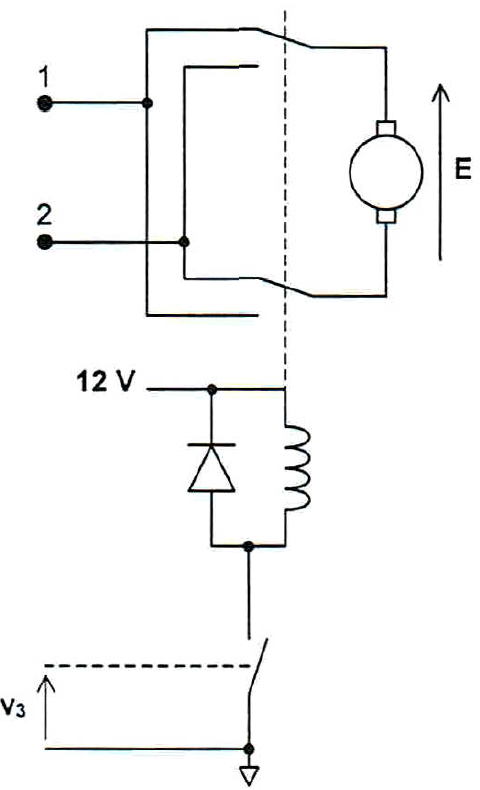
\includegraphics[width=.4\linewidth]{img/schema_elec2}
\end{center}
\caption{\label{schema_elec2}Système de relais pilotés}
\end{figure}

Au repos, lorsque la tension aux bornes de la bobine est nulle, les interrupteurs sont dans la position représentée sur la figure \ref{schema_elec2}. Lorsque la tension aux bornes de la bobine est égale à 12 V, les interrupteurs sont dans l'autre position.

\question{Quelle est l'utilité de ce système de relais ?}

\begin{figure}[ht!]
\begin{center}
 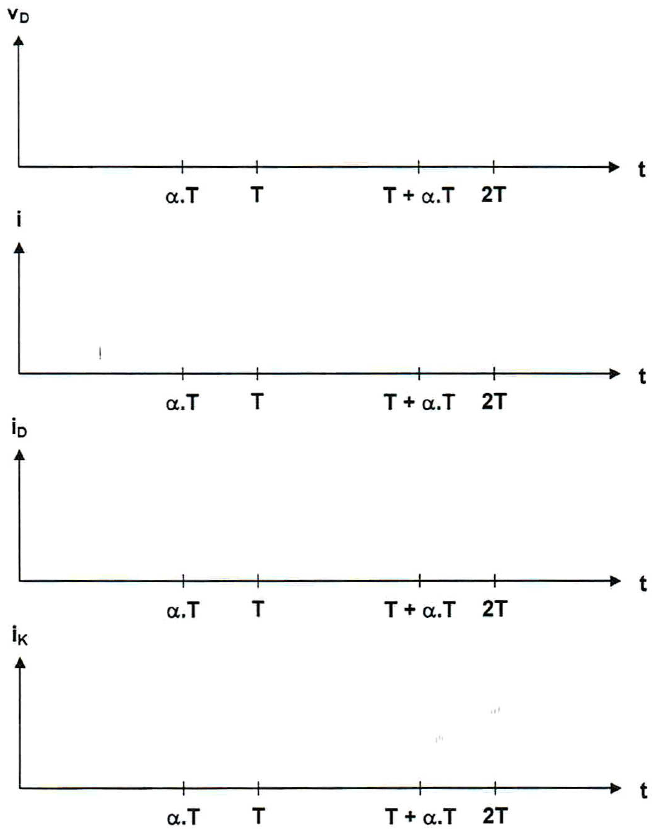
\includegraphics[width=.8\linewidth]{img/doc_reponse}
\end{center}
\end{figure}

\ifdef{\public}{\end{document}}{}

\newpage ~\ \newpage ~\


\pagestyle{correction}\setcounter{section}{0}

\reponse{$t\in[0,\alpha\cdot T]$ $V_s-L\cdot\dfrac{di(t)}{dt}-E=0$

$\dfrac{di(t)}{dt}=\dfrac{V_S-E}{L}$, donc $i(t)=\dfrac{V_S-E}{L}\cdot t+I_m$.

$t\in[\alpha\cdot T,T]$ 

$\dfrac{di(t)}{dt}=-\dfrac{E}{L}$, donc $i(t)=-\dfrac{E}{L}\cdot (t-\alpha\cdot T)+I_M$.}

\reponse{
\begin{figure}[ht!]
\begin{center}
  \def\svgwidth{.6\linewidth}
  \input{img/doc_reponse2.pdf_tex}\end{center}
\end{figure}}

\reponse{$<v_D(t)>=\int_0^T\dfrac{v(t)}{T}=\dfrac{\alpha\cdot V_s}{T}=\alpha\cdot V_S$

$<v_D(t)>=<L\cdot\dfrac{di(t)}{dt}>+<E>$

or $<L\cdot\dfrac{di(t)}{dt}>=0$ car $i(t)=i(t+T)$ et $<E>=E$ car vitesse constante, donc $E=\alpha\cdot V_s$.}

\reponse{$\Delta i=I_M-I_m$

On a $i(\alpha T)=\dfrac{V_s-E}{L}\cdot \alpha\cdot T+I_m=I_M$, donc $\Delta i=\dfrac{V_s-E}{L}\cdot \alpha T$.

E $i(T)=-\dfrac{E}{L}\cdot (T-\alpha\cdot T)+I_M=I_m$, donc $\Delta i=\dfrac{E}{L}\cdot (T-\alpha T)$.

Donc $(V_s-E)\cdot \alpha=E\cdot (1-\alpha)$, donc $V_S\cdot \alpha=E$, on retrouve bien l'équation précédente.}

\reponse{Tracé de $\Delta i=f(\alpha)$.}

\reponse{$\Delta i_{max}=\dfrac{V_s-E}{L}\cdot T$ pour $\alpha=1$.}

\reponse{$E=k\cdot N=\alpha\cdot V_s$, donc $\alpha=\dfrac{k\cdot N}{V_s}=\dfrac{5.25\cdot 10^{-2}\cdot 1000}{210}=\dfrac{52.5}{210}\approx 0,25$.}

\reponse{$t\in[0,\alpha\cdot T]$, donc $i_K=i$ et $i_D=0$

$t\in[\alpha\cdot T,T]$, donc $i_K=0$ et $i_D=i$

$<i_K(t)>=(I_M-I_m)\cdot\dfrac{\alpha\cdot T}{2}$

$<i_D(t)>=(I_M-I_m)\cdot\dfrac{T-\alpha\cdot T}{2}$.}

\reponse{Cela permet de changer le sens de rotation.}

\end{document}